\documentclass[acmtog]{acmart}

%% Rights management information.  This information is sent to you
%% when you complete the rights form.  These commands have SAMPLE
%% values in them; it is your responsibility as an author to replace
%% the commands and values with those provided to you when you
%% complete the rights form.
\setcopyright{none}
% \copyrightyear{2024}
% \acmYear{2024}
% \acmDOI{XXXXXXX.XXXXXXX}


%%
%% These commands are for a JOURNAL article.
\acmJournal{TOG}
\acmVolume{X}
\acmNumber{X}
\acmArticle{X}
\acmMonth{12}

%%
%% Submission ID.
%% Use this when submitting an article to a sponsored event. You'll
%% receive a unique submission ID from the organizers
%% of the event, and this ID should be used as the parameter to this command.
%%\acmSubmissionID{123-A56-BU3}

%%
%% For managing citations, it is recommended to use bibliography
%% files in BibTeX format.
%%
%% You can then either use BibTeX with the ACM-Reference-Format style,
%% or BibLaTeX with the acmnumeric or acmauthoryear sytles, that include
%% support for advanced citation of software artefact from the
%% biblatex-software package, also separately available on CTAN.
%%
%% Look at the sample-*-biblatex.tex files for templates showcasing
%% the biblatex styles.
%%

%%
%% The majority of ACM publications use numbered citations and
%% references.  The command \citestyle{authoryear} switches to the
%% "author year" style.
%%
%% If you are preparing content for an event
%% sponsored by ACM SIGGRAPH, you must use the "author year" style of
%% citations and references.
\citestyle{acmauthoryear}


%%
%% end of the preamble, start of the body of the document source.
\begin{document}

%%
%% The "title" command has an optional parameter,
%% allowing the author to define a "short title" to be used in page headers.
\title{3D Human Texture Estimation from a Single Image}

%%
%% The "author" command and its associated commands are used to define
%% the authors and their affiliations.
%% Of note is the shared affiliation of the first two authors, and the
%% "authornote" and "authornotemark" commands
%% used to denote shared contribution to the research.
\author{Ziyao Wang}
\affiliation{
  \institution{University of British Columbia}
  \city{Vancouver}
  \state{BC}
  \country{Canada}
}
\email{zwubc@ece.ubc.ca}

%%
%% By default, the full list of authors will be used in the page
%% headers. Often, this list is too long, and will overlap
%% other information printed in the page headers. This command allows
%% the author to define a more concise list
%% of authors' names for this purpose.
\renewcommand{\shortauthors}{Ziyao Wang}

%%
%% The abstract is a short summary of the work to be presented in the
%% article.
\begin{abstract}
  The paper SMPLitex \cite{casas2023smplitex} proposed a fine-tuned \texttt{stable-diffusion-v1-4} model for 3D human texture estimation from a single image. The SMPLitex model can generate a 512x512 texture of SMPL UV map from a text prompt or reconstruct a full texture based on a partial texture created from a single image. The texture is then applied to SMPL meshes for 3D rendering tasks. Although SMPLitex used image refinement tools to produce impressive results compared with the prior works, it also introduced inpainting inconsistency to its generated textures. In this paper, I used DreamBooth to fine-tune \texttt{stable-diffusion-2-inpainting} model with training images selected from SMPLitex dataset and training masks generated from DeepFashion-MultiModal dataset. With subjective analysis, I concluded that my fine-tuned model is much more consistent in inpainting than the SMPLitex model. With quantitative analysis such as SSIM and LPIPS, I concluded that my model does better in texture reconstruction than the SMPLitex one.
\end{abstract}

%%
%% The code below is generated by the tool at http://dl.acm.org/ccs.cfm.
%% Please copy and paste the code instead of the example below.
%%
\begin{CCSXML}
  <ccs2012>
  <concept>
  <concept_id>10010147.10010178.10010224.10010245.10010254</concept_id>
  <concept_desc>Computing methodologies~Reconstruction</concept_desc>
  <concept_significance>500</concept_significance>
  </concept>
  </ccs2012>
\end{CCSXML}

\ccsdesc[500]{Computing methodologies~Reconstruction}

%%
%% Keywords. The author(s) should pick words that accurately describe
%% the work being presented. Separate the keywords with commas.
\keywords{Stable Diffusion, DreamBooth, SMPL, DensePose}

%%
%% This command processes the author and affiliation and title
%% information and builds the first part of the formatted document.
\maketitle

\section{Introduction}

The paper SMPLitex \cite{casas2023smplitex} proposed a fine-tuned \texttt{stable-diffusion-v1-4} model for 3D human texture estimation from a single image. The SMPLitex model is a general stable diffusion model with two typical use cases: \texttt{text2image} and \texttt{image2image}. The former generates a texture from a text prompt, while the latter generates a texture from another texture. The SMPLitex model is fine-tuned with DreamBooth such that its generated textures fit in the unwrapped UV map of SMPL human model. DensePose \cite{guler2018densepose} is a technique to map all human pixels of a 2D image to the 3D surface of human body. With the help of DensePose, one can create a partial texture (due to FoV blocking) from a single image, and the partial texture becomes the input of \texttt{image2image} task to reconstruct a full texture. That is the general idea of the SMPLitex paper.

This paper fine-tuned \texttt{stable-diffusion-2-inpainting} model based on the idea of the SMPLitex paper above. The base model is an inpainting-specialized stable diffusion model with only one use: \texttt{inpainting}. Compared with the \texttt{image2image} task, \texttt{inpainting} takes a partial texture as well as an inpainting mask as input and only reconstruct the masked area (holes and missing parts except the texture area) in the partial texture. This ensures the original partial texture is not altered after inpainting. On the contrary, \texttt{image2image} generates a new texture for several denoising steps with the partial texture as the initial noise image. During the denoising process, the partial texture is distorted greatly. As a workaround, the \texttt{image2image} output is masked with the original partial texture to ensure the original texture area remains constant. This branch of \texttt{image2image} used by SMPLitex is also known as \texttt{legacy\_inpaint}. It is now deprecated because its inpainted area is inconsistent with the original texture area. With such constraint, I can see from the results in the SMPLitex paper that the front and back colors of the clothes on a rendered 3D human are different.

\begin{figure}[h]
  \centering
  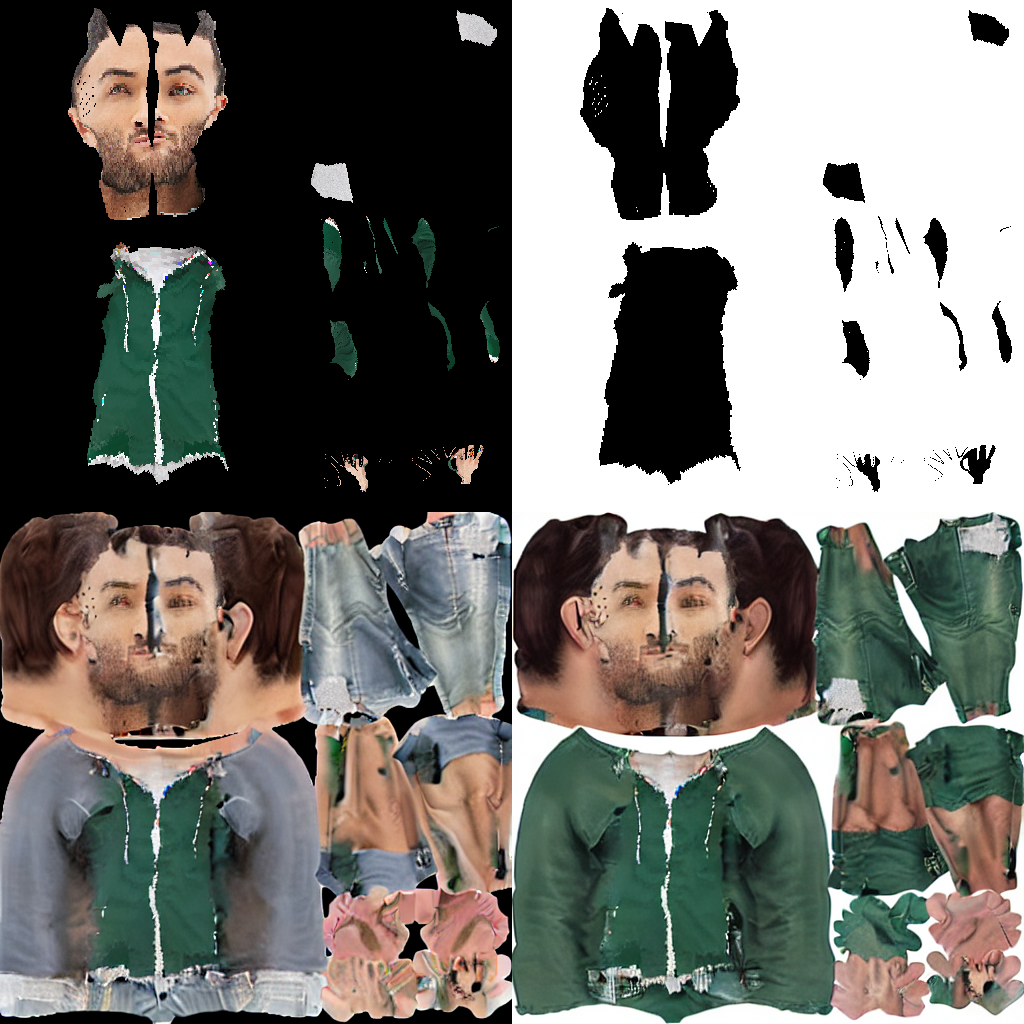
\includegraphics[width=0.47\textwidth]{figs/smplitex_sample.png}
  \caption{SMPLitex-generated examples.}
  \Description{SMPLitex sample.}
  \label{fig:smplitex_sample}
\end{figure}

As shown in Fig \ref{fig:smplitex_sample}, the top left is a partial texture, the top right is its inpainting mask, the botton left is legacy inpainted texture using SMPLitex model without any image refinement techniques, and the bottom right is legacy inpainted texture with text ``green'' appended into the prompt so that the inpaint area is at least in a similar color compared with the original texture area. However, one can distinguish the original and inpaint textures even in the bottom right image, and the face reconstruction is bad in the SMPLitex model. Actually, SMPLitex used CodeFormer \cite{zhou2022towards} to restore faces in their results.

My work in this paper addressed the issue of the SMPLitex model above. I used DreamBooth to fine-tune stable-diffusion-2-inpainting model. Unlike general models, the training dataset for an inpainting model includes images as well as masks. The training images were selected from the SMPLitex dataset and training masks were generated using DensePose from DeepFashion-MultiModal dataset \cite{jiang2022text2human}. Note that fine-tuning an inpainting model is also possible with only training images, where the training masks are generated randomly using algorithms during training. However, in this way, the inpainting areas masked will be random and the model will perform unsatisfyingly in inference, based on my experiment results.

For results comparison, SSIM and LPIPS metrics were adopted because of their approximation to human perception.

\section{Related Work}

Several remarkable works on machine learning form the foundation of my work. The paper would be infeasible without them.

\subsection{Stable Diffusion}

Stable diffusion is a latent diffusion model that can generate images from random noise using text-guided denoising schedulers. A stable diffusion model has three components: variational autoencoders/autodecoders (VAE), a text encoder (CLIP), and a U-Net.

\begin{itemize}
  \item VAE produces input varied in dimension as output. VAE encoders reduce the dimension of input, and VAE decoders increase the dimension of input. A 512x512 image has 3x512x512 dimensions (3 for RGB channels), which will result in curse of dimensionality without proper encoding.
  \item CLIP encodes the input text prompt as text embedding vectors to use in U-Net.
  \item U-Net performs denoising guided by text embeddings. Fine-tuning a stable diffusion model is actually training only the last few layers (for simplicity) of the U-Net in it.
\end{itemize}

First, a randomly-generated pure noise image goes through several VAE encoders to downscale and reduce dimensionality. Then, it is denoised with a U-Net guided by CLIP-encoded text embeddings. Finally, the output image goes through several VAE decoders to upscale and restore its dimentionality.

\subsection{DensePose}

DensePose (dense human pose estimation) \cite{guler2018densepose} is a pipeline with trained models to map all human pixels of an 2D image to the 3D surface of the human body. It is such important that it connects a 2D image of human to a partial texture of Atlas UV map and assigns pixels accurately to different parts of the UV map.

DensePose stores the mapping of pixels to parts in IUV images. The DensePose IUV image stores indexes and UV coordinates of pixels in a 2D image. For each pixel, the index I is an integer in \([0,24]\) (24 human parts + 1 background) and the U\&V are float numbers in \((0,1)\) indicating relative coordinate of the pixel in that human part (for background pixel \(I==0\), UV are zeros).

The UV map compatible with DensePose is Atlas, with 24 human parts arranged in a \(6x4\) grid. Nonetheless, the illogical arrangement of human parts in Atlas makes its inpainting more difficult than SMPL, and converting Atlas to SMPL UV map is quite easy. Therefore, I fine-tuned the model based on SMPL textures.

\subsection{Semantic Guided Human Matting}

Semantic Guided Human Matting \cite{chen2022robust} is a semantic segmentation model specifically trained for human. It is very robust and accurate in removing the background of a portrait. In the paper, it is used together with DensePose to generate the masked DensePose IUV images.

\begin{figure}[h]
  \centering
  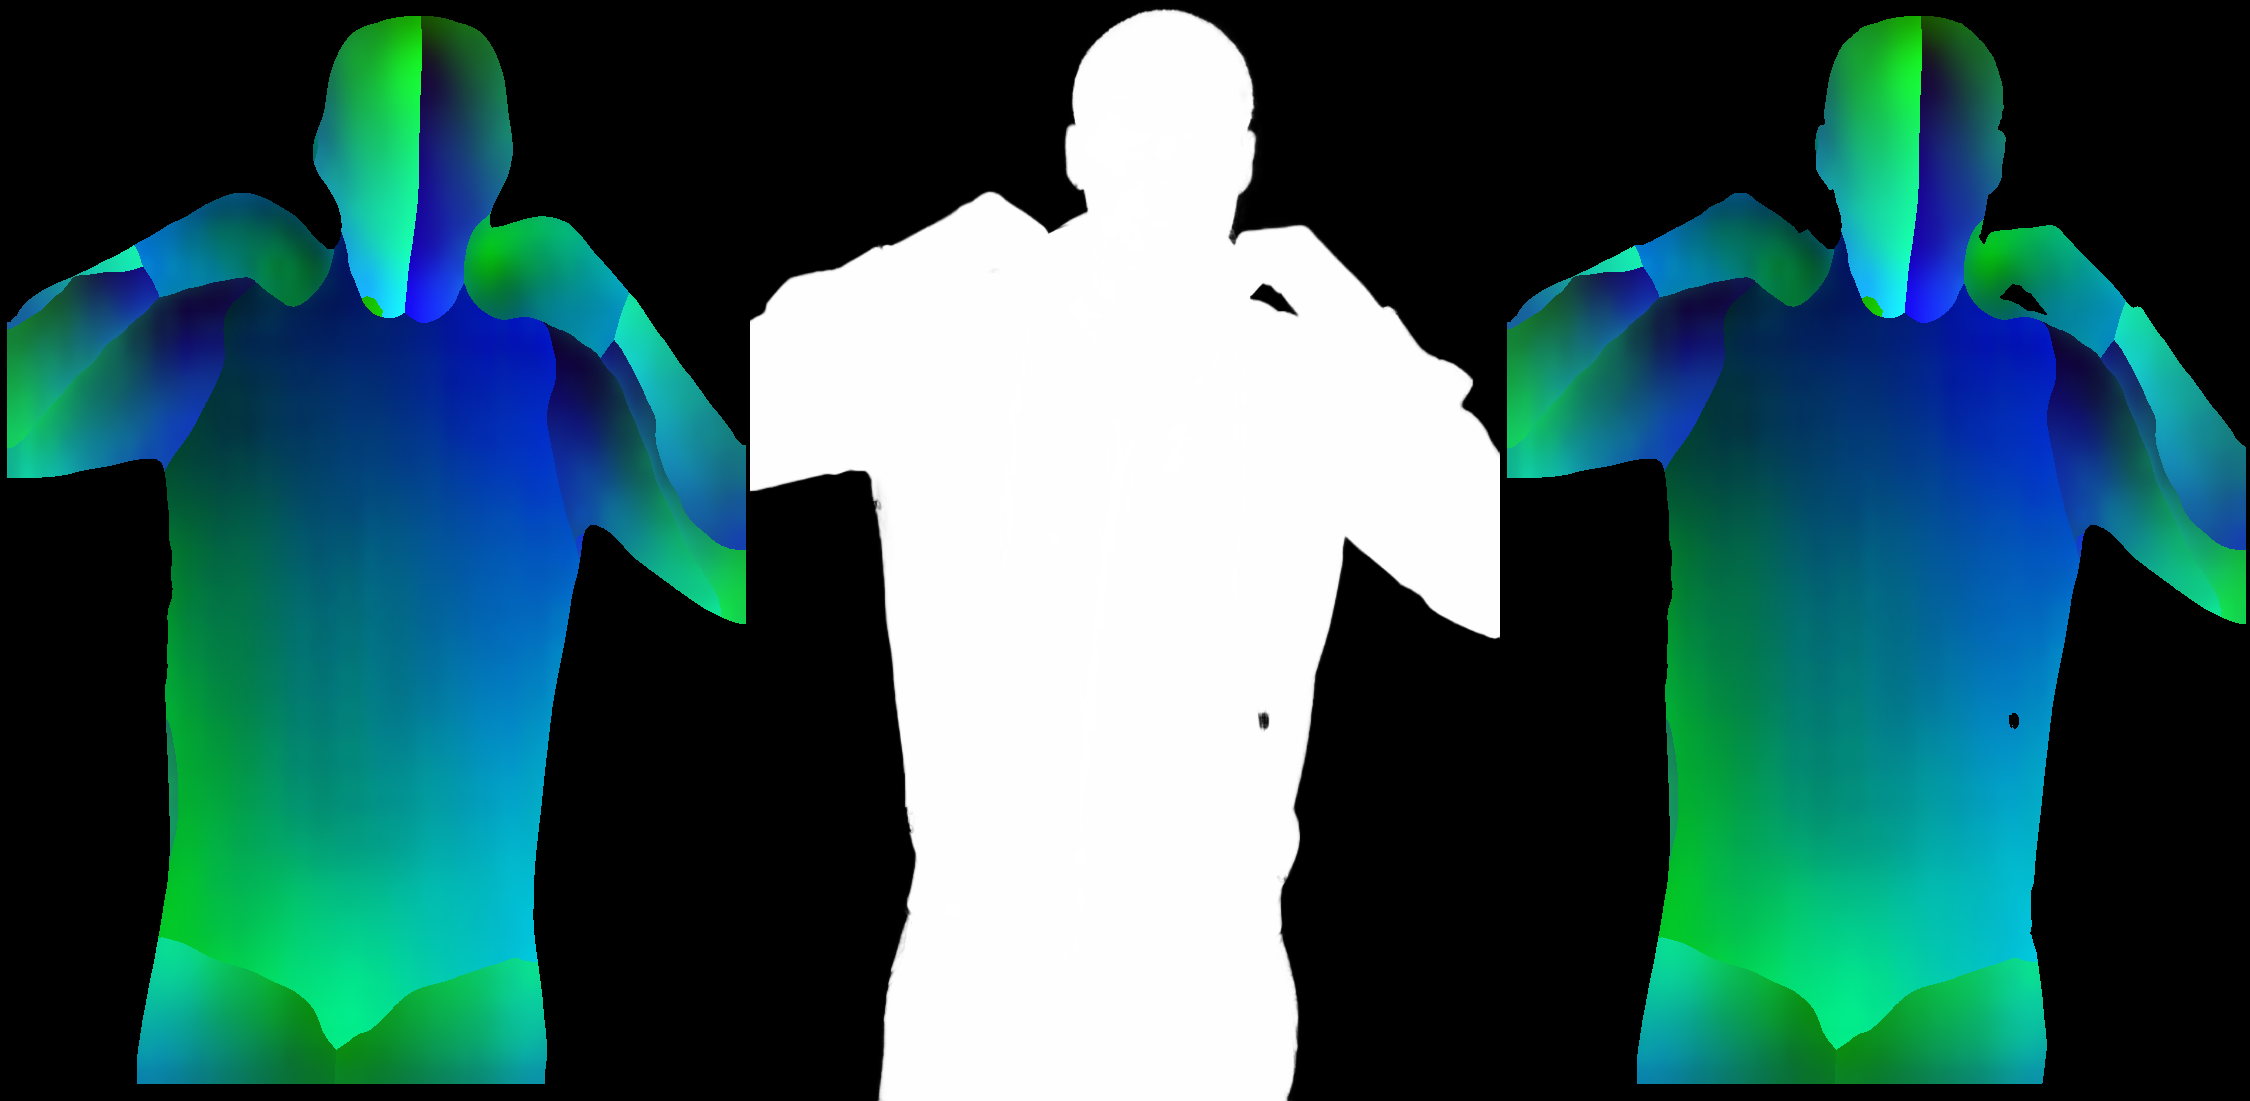
\includegraphics[width=0.47\textwidth]{figs/human_matting.png}
  \caption{Use of Semantic Guided Human Matting.}
  \Description{Use of Semantic Guided Human Matting.}
  \label{fig:human_mat}
\end{figure}

As shown in Fig \ref{fig:human_mat}, the left is a DensePose IUV image, the middle is a human mat, and the right is the composite of them (masked DensePose IUV image). Since DensePose is not good at accurate separation of human and background, I used Semantic Guided Human Matting to mask the DensePose IUV image and remove background edges. You can see from the right IUV image the clear edges of ears and hands.

\subsection{DreamBooth}

DreamBooth \cite{ruiz2023dreambooth} is a technique to fine-tune stable diffusion models with very few training data (typically 3-5 images) and a text identifier. The aim is to instruct the model to generate only certain style of images when the idenfier is in the text prompt, like the texture of SMPL UV map.

To avoid overfitting and loss of prior knowledge, the selected identifier (``sks'' in DreamBooth paper) has least relation to existing text embeddings. In a fine-tuned model, the prompt ``a texture'' can means any textures, while the prompt ``a sks texture'' instructs the model to generate only textures of the SMPL UV map.

\section{Methods}

The methods are for quantitative comparision of my model with SMPLitex model.

\subsection{SSIM}

SSIM (structural similarity index measure) is a well-known method to measure structural similarity of two images. Unlike the common MSE (mean square error), SSIM focuses on the inter-dependency of pixels close to each other, which carries the structure information of the image.

Equation 1 is the formula of SSIM, where \(\mu\) represents pixel sample mean, \(\sigma_{xy}\) is covariance, and constant \(c_1\) and \(c_2\) help smooth the SSIM value and avoid zero division.

\begin{equation}
  SSIM(x,y)=\frac{(2\mu_x\mu_y+c_1)(2\sigma_{xy}+c2)}{({\mu_x}^2+{\mu_y}^2+c_1)({\sigma_x}^2+{\sigma_y}^2+c_2)}
\end{equation}

SSIM score is similar to human perception. The range of SSIM is \([-1,1]\), where 0 indicates no similarity, 1 is structural identical, and -1 is perfect anti-correlation.

However, SSIM is vulnerable to compression, so it may not perform well when comparing compressed JPGs obtained from the Internet.

\subsection{LPIPS}

LPIPS (learned perceptual image patch similarity) \cite{zhang2018unreasonable} is a deep-learning based metric to compare two images perceptually like human. It provides a Python package and helper methods ready to use in our project. Higher score means more different, and lower score (approx 0) means more similar perceptually.

\section{Fine-tuning}

Fune-tuning \texttt{stable-diffusion-2-inpainting} requires both images and masks in the training dataset.

\subsection{Preparing Training Data}

For training images, I selected 12 textures of SMPL UV map from SMPLitex dataset. The SMPLitex dataset is a collection of high-quality textures generated by SMPLitex model via \texttt{text2image}.

\begin{figure}[h]
  \centering
  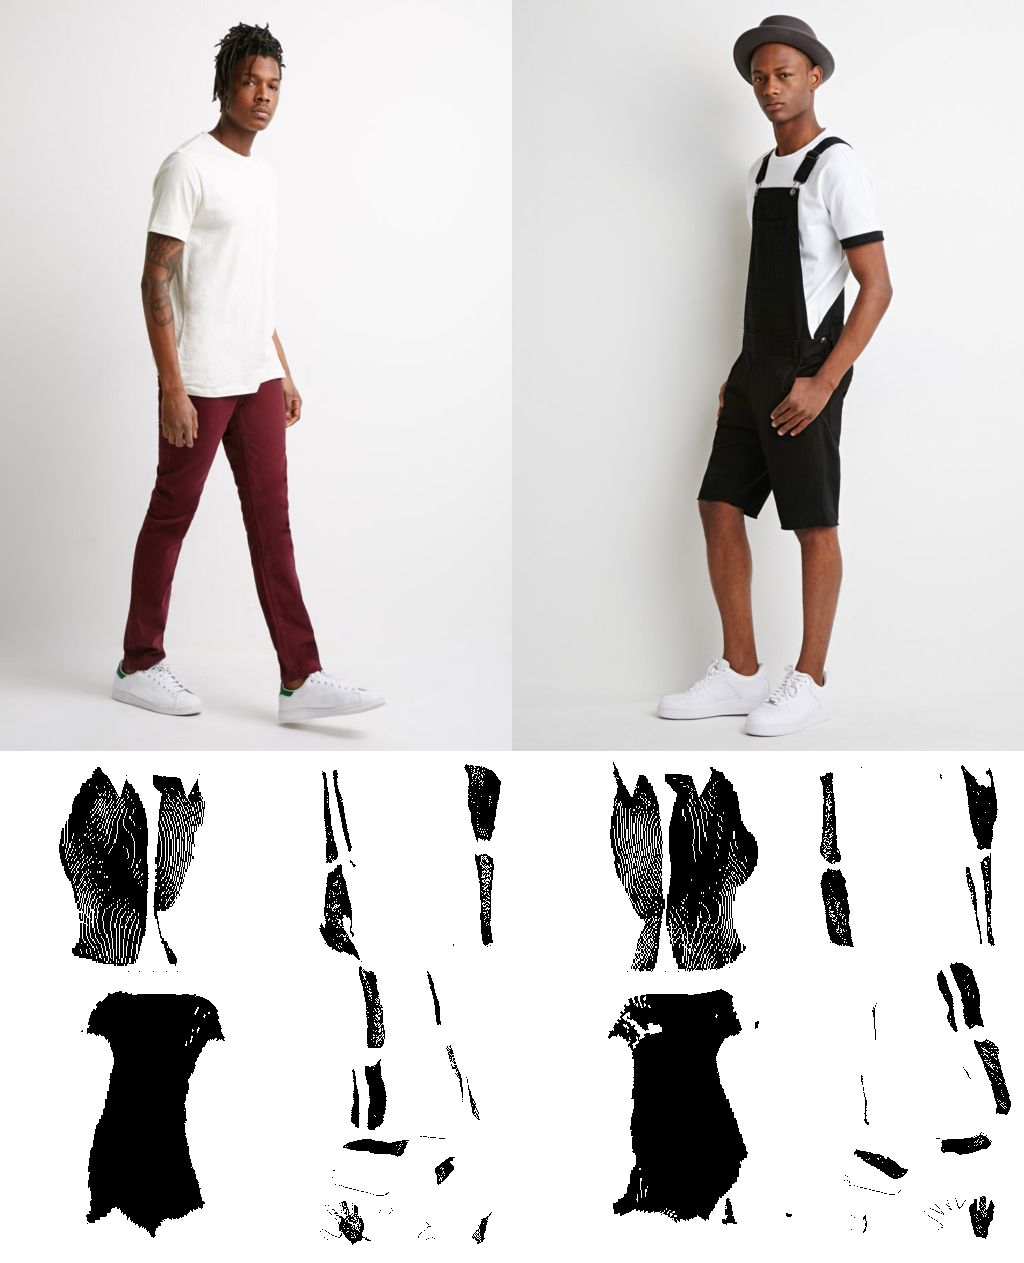
\includegraphics[width=0.47\textwidth]{figs/training_mask.png}
  \caption{Creation of training masks.}
  \Description{Creation of training masks.}
  \label{fig:train_mask}
\end{figure}

The training masks were created from DeepFashion-MultiModal dataset \cite{jiang2022text2human}. I selected 10 images from the dataset and created 10 texture masks of SMPL UV map from them. Fig \ref{fig:train_mask} shows two of the masks and their source images. Note that due to mapping and scaling, there are numerous strip-shaped holes in the masks. The SMPLitex paper suggests to blur the masks to get rid of the holes to achieve better inpainting results. I kept the holes in training because in this way the model could learn to also reconstruct human faces.

\subsection{Modifying the Fine-tuning Script}

The Diffusers \cite{von-platen-etal-2022-diffusers} is a Python library for state-of-the-art pretrained diffusion models for generating images and other media. It offers on its GitHub repository a dozens of Python scripts to fine-tune stable diffusion models with DreamBooth using Diffusers. The \href{https://github.com/huggingface/diffusers/blob/main/examples/research\_projects/dreambooth\_inpaint/train\_dreambooth\_inpaint.py}{\texttt{train\_dreambooth\_inpaint.py}} script fine-tunes an inpaint model with only training images. The script creates random masks using rectangles and circles during training. However, this approximation of training masks is coarse and will make fine-tuned model unable to inpaint correctly, based on my experiment.

To overcome the issue, I modified the script so that it chose randomly a mask from all training masks to pair with the selected training image every training step. In this way, the model could learn to inpaint my desired areas during training while the randomness of training data was preserved.

\subsection{Tuning Hyper-parameters}

I started from the hyper-parameters used in the SMPLitex paper, and modified them based on fine-tuned model performance. It is worth mentioning some of the hyper-parameters.

\begin{itemize}
  \item \texttt{max\_train\_steps}=1500
  \item[] The number of training steps is converted to the number of epochs during training. A epoch indicates a full visit of all training images.
  \item \texttt{gradient\_accumulation\_steps}=2
  \item[] It is the number of update steps to accumulate before doing a backward propagation. Larger value means more stable training at the cost of larger VRAM usage.
  \item \texttt{lr\_scheduler}='constant'
  \item[] The learning rate scheduler specifies how the learning rate changes with steps. Constant learning rate is more suitable in generative models when the loss function plays a less important role.
  \item \texttt{learning\_rate}=1e-6
  \item[] The learning rate in DreamBooth should be smaller than other machine learning tasks to prevent overfitting the small training dataset.
\end{itemize}

I recorded the training loss on tensorboard, as shown in Fig \ref{fig:train_loss}. Note that the lines in the graph were already smoothened. From my previous machine learning experience, an oscillating loss means unsuccessful training. But, for generative models like stable diffusion, which I realized later, the loss function shouldn't converge to 0. A zero loss means perfect inpainting the training images and perfect overfitting. A generative model should have the generalization ability to create various images given the same prompt, and this ability can explain the oscillation of the loss function.

I also fine-tuned the model with a smaller learning rate 1e-7 to expect less oscillation, but its loss function was very similar to Fig \ref{fig:train_loss} and from inpaint testing, the fine-tuned model actually didn't learn.

\begin{figure}[h]
  \centering
  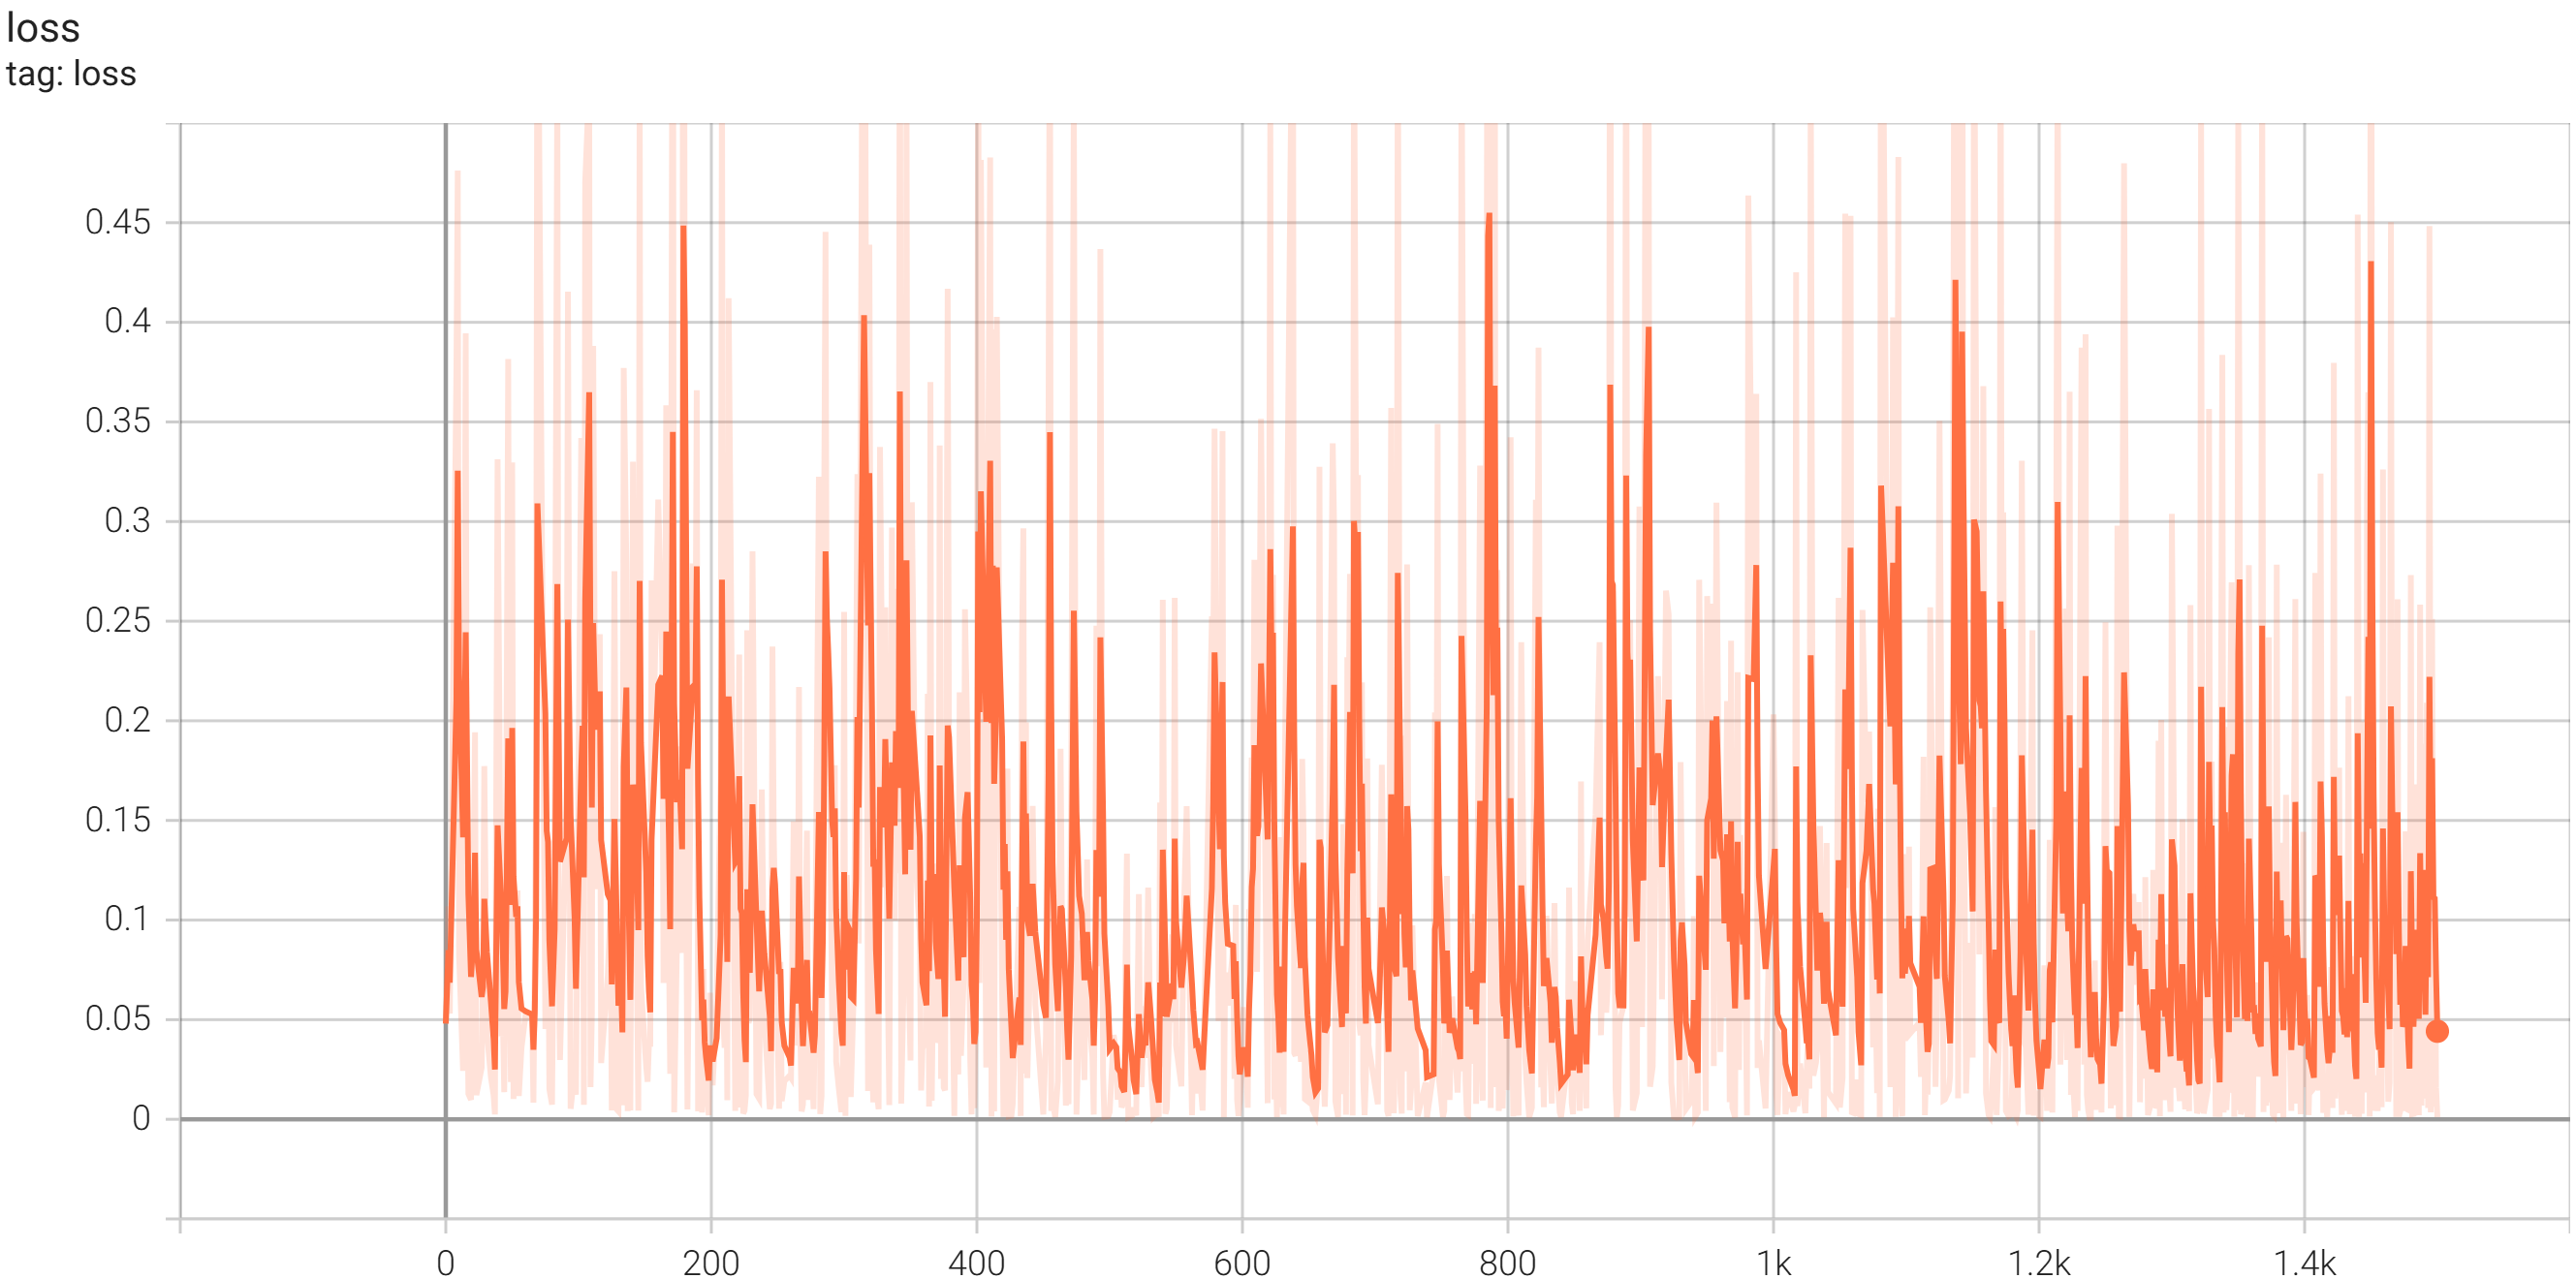
\includegraphics[width=0.47\textwidth]{figs/training_loss.png}
  \caption{Fine-tuning loss.}
  \Description{Fine-tuning loss.}
  \label{fig:train_loss}
\end{figure}

\section{Results}

My fine-tuned model performed better than I expected. Fig \ref{fig:inpaint_result} shows three examples in the inpainting test without any postprocessing. Not only could the model inpaint in consistency, but the model could also restore the faces by filling strip-shaped holes to some extent.

The text prompt was ``a smpl texture'' where I used ``smpl'' as the unique identifier to distinguish smpl textures from general textures. Other texts including colors were not used. With subjective analysis, the inpainting areas and the original texture areas blended smoothly, which outperformed the SMPLitex model.

Using quantitative analysis, I calculated the average SSIM and LPIPS of the results generated by the two models based on the DeepFashion-MultiModal and SMPLitex dataset. The SSIM algorithm used \texttt{window\_size}=7, \texttt{K1}=0.01, and \texttt{K2}=0.03, while LPIPS used its default hyper-parameters. The results are shown below.

\begin{table}[h]
  \caption{SSIM and LPIPS}
  \label{tbl:results}
  \begin{tabular}{ccc}
    \toprule
    Average & SSIM & LPIPS \\
    \midrule
    Mine & 0.7290 & 0.6356 \\
    SMPLitex & 0.3675 & 0.4942 \\
    \bottomrule
  \end{tabular}
\end{table}

From Table \ref{tbl:results}, my fine-tuned model outperforms the SMPLitex model in both SSIM amd LPIPS. Considering the difference, SSIM is more concrete and it focuses on the structures in blocks, while LPIPS is more perceptual and it tends to ignore the slight differences and focuses on the big changes.

\begin{figure}[h]
  \centering
  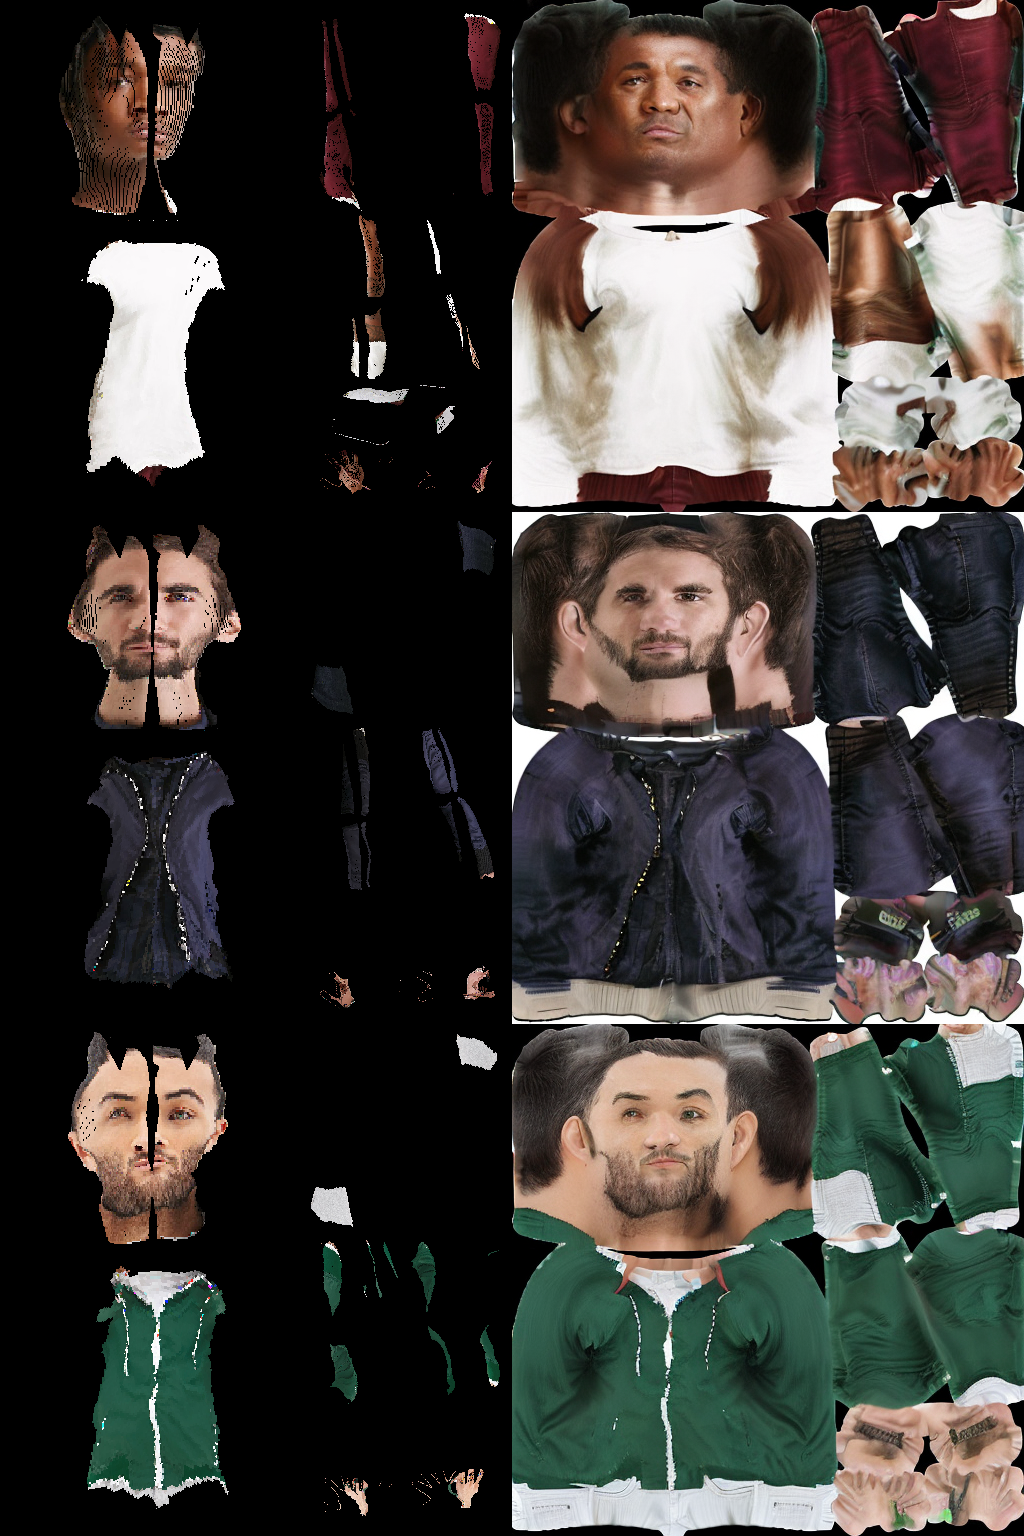
\includegraphics[width=0.47\textwidth]{figs/inpaint_results.png}
  \caption{Inpaint results.}
  \Description{Inpaint results.}
  \label{fig:inpaint_result}
\end{figure}

\section{Conclusion}

In the project, I discussed the SMPLitex paper and their work, and fine-tuned the \texttt{stable-diffusion-2-inpainting} model based on their ideas. With quantitative analysis, my model outperformed theirs in all metrics.

The possible future work includes using lora to fine-tune the latest \texttt{stable-diffusion-3-inpainting} model, and applying various preprocessing and postprocessing techniques to make inpainting more stable.


%%
%% The next two lines define the bibliography style to be used, and
%% the bibliography file.
\bibliographystyle{ACM-Reference-Format}
\bibliography{report}


%%
%% If your work has an appendix, this is the place to put it.
\appendix

\section{Project Codes}

Available on GitHub:

\href{https://github.com/wangziyao318/img2tex}{\texttt{https://github.com/wangziyao318/img2tex}}

\end{document}
\endinput
